%% ============================================================
%%  AttnFuse: A Composable Python DSL for Compiling Attention
%%             to Fused Triton Kernels
%%
%%  Draft for an MLSys-class submission. Self-contained: builds
%%  with pdflatex out of the box. Figures live alongside this
%%  .tex; CSVs the numbers come from live under results/.
%% ============================================================
\documentclass[10pt,twocolumn]{article}

\usepackage[margin=0.75in,top=0.9in,bottom=0.9in]{geometry}
\usepackage[T1]{fontenc}
\usepackage{lmodern}
\usepackage{microtype}
\usepackage{amsmath,amssymb}
\usepackage{graphicx}
\usepackage{booktabs}
\usepackage{multirow}
\usepackage{array}
\usepackage{float}
\usepackage{subcaption}
\usepackage{listings}
\usepackage{xcolor}
\usepackage[colorlinks=true,linkcolor=blue!60!black,
            citecolor=blue!60!black,urlcolor=blue!60!black]{hyperref}
\usepackage{parskip}
\usepackage{enumitem}
\usepackage{balance}

\definecolor{codebg}{HTML}{F8F8F8}
\definecolor{codeframe}{HTML}{CCCCCC}
\definecolor{kwcol}{HTML}{0000CC}
\definecolor{comcol}{HTML}{008000}
\definecolor{strcol}{HTML}{CC0000}
\lstset{
  language=Python,
  backgroundcolor=\color{codebg},
  frame=single,
  rulecolor=\color{codeframe},
  basicstyle=\ttfamily\scriptsize,
  keywordstyle=\color{kwcol}\bfseries,
  commentstyle=\color{comcol}\itshape,
  stringstyle=\color{strcol},
  breaklines=true,
  showstringspaces=false,
  tabsize=2,
  captionpos=b,
}

\title{%
  \textbf{AttnFuse: A Composable Python DSL for Compiling\\
  Attention Variants to Fused Triton GPU Kernels}\\[6pt]
  \large Forward, Backward, KV-cache Decoding, and Block-Sparse Training
}
\author{Varun Kumar Dasoju}
\date{\today}

\begin{document}
\maketitle

%% =============================================================
\begin{abstract}
%% =============================================================
Modern attention research increasingly invents new score, mask, and
positional-encoding combinations--sliding-window, ALiBi, Rotary Position
Embeddings (RoPE), block-sparse--each of which today requires hand-written
CUDA or Triton to run efficiently on a GPU. We present \textbf{AttnFuse},
a small embedded Python DSL that lets a user describe an attention variant
declaratively using composable combinators and compiles the description to
a single fused Triton kernel via a two-level intermediate representation.
A four-pass compiler fuses score, mask, bias, normalisation, and
value-weighted aggregation into one tiled online-softmax loop, achieving
IO-complexity identical to FlashAttention-2. AttnFuse covers the full LLM
training-and-inference stack: forward inference, autoregressive KV-cache
decoding (via a tensor-core-aware Flash Decoding kernel with cyclic
Q-head replication for Grouped-Query Attention), training (via an
FA2-style backward kernel wired through \texttt{torch.autograd.Function}),
and block-sparse attention (BigBird-style with both forward and backward
kernels operating on user-supplied active-block lists). On an NVIDIA RTX
3090, AttnFuse matches PyTorch's \texttt{flex\_attention} within 5--6\%
on supported variants, wins every Rotary-Position-Embedding (RoPE)
composition cell by up to $2.10\times$ (RoPE structurally cannot be
expressed in \texttt{flex\_attention}'s \texttt{score\_mod} hook), wins
every KV-cache decoding cell across three production-LLM geometries, and
runs a real HuggingFace Llama-3-8B \texttt{LlamaDecoderLayer} training
step at $1.06\times$ of PyTorch SDPA. Correctness is established by 100
GPU unit tests plus a Hypothesis-driven property fuzzer (80 randomised
configurations per run, zero failures).
\end{abstract}

%% =============================================================
\section{Introduction}
%% =============================================================

Multi-head self-attention dominates the compute and memory budget of
modern Transformer models. The standard PyTorch implementation
decomposes attention into a sequence of discrete kernels--$QK^\top$,
scale, mask, softmax, attention-times-V--each materialising an
$\mathcal{O}(N^2)$ intermediate in high-bandwidth memory (HBM).
FlashAttention~\cite{dao2022flashattention,dao2023flashattention2} (FA2)
collapses these into a single fused kernel using an online softmax
recurrence, reducing HBM reads from $\mathcal{O}(N^2)$ to
$\mathcal{O}(N^2 d / M)$ where $M$ is on-chip SRAM. FA2 is, however,
hand-written CUDA for a fixed set of variants (dense, causal); the
moment a researcher wants sliding-window~\cite{child2019generating},
ALiBi~\cite{press2021alibi}, fused
RoPE~\cite{su2021roformer}, block-sparse~\cite{zaheer2020bigbird}, or
any composition of these, the FA2 binary cannot help.

PyTorch's recent \texttt{flex\_attention} API (PyTorch 2.5)
addresses some of this gap by accepting a user-supplied Python
\texttt{score\_mod} function and emitting a fused Triton kernel through
TorchInductor. But \texttt{flex\_attention}'s \texttt{score\_mod} hook
fires \emph{after} the $QK^\top$ matmul, which means any positional
encoding that must be applied to $Q$ and $K$ \emph{before} the
matmul--most notably RoPE--cannot be fused. RoPE, paradoxically the
positional encoding used by every major recent LLM (LLaMA, Mistral,
Falcon, Qwen, DeepSeek), is the largest single gap in
\texttt{flex\_attention}'s coverage.

We introduce \textbf{AttnFuse}, an embedded Python DSL for attention
that compiles to fused Triton kernels via a small two-level IR. The
user writes attention as a short function using composable combinators
(\texttt{scaled\_dot\_product}, \texttt{rope}, \texttt{causal},
\texttt{sliding\_window}, \texttt{alibi}, \texttt{block\_sparse},
\texttt{softmax}); a four-pass compiler emits a single parameterised
Triton kernel that is specialised per \texttt{tl.constexpr} combination,
giving zero runtime branching.

\paragraph{Contributions.}
\begin{itemize}[leftmargin=1.2em,itemsep=1pt]
  \item A composable DSL with eight combinators captured by symbolic
        tracing into a typed dataflow IR (\S\ref{sec:dsl}).
  \item A two-level IR plus four-pass compiler emitting a single
        parameterised Triton kernel (\S\ref{sec:compiler}).
  \item A novel \textbf{fused-RoPE kernel} that rotates Q and K
        tiles inside the inner loop, a capability not expressible
        in \texttt{flex\_attention}'s post-matmul \texttt{score\_mod} hook
        (\S\ref{sec:rope}).
  \item A \textbf{Flash Decoding kernel} for autoregressive KV-cache
        inference, with cyclic Q-head replication recovering tensor-core
        throughput for Grouped-Query Attention (\S\ref{sec:decode}).
  \item A complete \textbf{FA2-style backward pass} wired through
        \texttt{torch.autograd}, enabling training on every supported
        variant including GQA and block-sparse (\S\ref{sec:backward},
        \S\ref{sec:blocksparse}).
  \item A \textbf{block-sparse training} path with a CSR-style
        \texttt{BlockMask} abstraction that yields genuinely
        sub-quadratic FLOPs in proportion to the active-tile fraction
        (\S\ref{sec:blocksparse}).
  \item A comprehensive evaluation on RTX 3090 (Ampere) and H100
        (Hopper) showing AttnFuse matches or beats PyTorch
        \texttt{flex\_attention} on every variant it supports on
        Ampere, wins every RoPE composition cell, wins every KV-cache
        decoding cell, and runs a real Llama-3-8B training step within
        6--11\% of PyTorch SDPA (\S\ref{sec:eval}).
\end{itemize}

%% =============================================================
\section{Background}
\label{sec:background}
%% =============================================================

\paragraph{FlashAttention and online softmax.}
The key idea of FlashAttention is the online softmax recurrence of
Milakov and Gimelshein~\cite{milakov2018online}: the numerically stable
softmax can be computed by maintaining a per-row running max $m_i$ and
running sum $\ell_i$, updating both as each key-value tile arrives. The
attention output can then be computed in a single nested loop without
ever materialising the full $N \times N$ score matrix.

\paragraph{Triton.}
Triton~\cite{tillet2019triton} is a Python-embedded GPU DSL whose JIT
compiler accepts \texttt{tl.constexpr} arguments that are specialised
at the Python level before PTX code generation. This enables
zero-overhead variant dispatch without runtime branching, which AttnFuse
relies on heavily.

\paragraph{Grouped-Query Attention.}
Modern LLMs (Llama 3, Mistral, Falcon) use GQA: the $Q$ tensor has
$H_q$ query heads but $K$ and $V$ have only $H_{kv}$ heads, with each
KV head shared by $H_q / H_{kv}$ query heads. The extreme case
$H_{kv} = 1$ is Multi-Query Attention (MQA, used by Falcon, PaLM).

\paragraph{Rotary Position Embeddings.}
RoPE~\cite{su2021roformer} encodes token position by rotating $Q$ and
$K$ by a position-dependent angle \emph{before} the score matmul. This
``before the matmul'' property is what makes RoPE structurally
inexpressible in \texttt{flex\_attention}'s post-matmul \texttt{score\_mod} hook.

%% =============================================================
\section{System Design}
%% =============================================================

\subsection{The Composable DSL}
\label{sec:dsl}

AttnFuse exposes eight composable combinators that snap together inside
an \texttt{@af.attention}-decorated Python function. The decorator
traces the function once with symbolic \texttt{TensorSym} placeholders;
each combinator call returns an IR node, building a typed dataflow
graph without running any GPU code.

\begin{lstlisting}[caption={GPT-2-style causal attention in five lines of AttnFuse DSL.}]
import attnfuse as af

@af.attention
def gpt2_attn(Q, K, V):
    s = af.scaled_dot_product(Q, K)
    s = af.causal(s)
    return af.softmax(s) @ V

out = gpt2_attn(Q, K, V)  # JIT-compiles a fused Triton kernel
\end{lstlisting}

The eight combinators are: \texttt{scaled\_dot\_product},
\texttt{rope} (fused RoPE), \texttt{causal}, \texttt{sliding\_window},
\texttt{full}, \texttt{block\_sparse}, \texttt{alibi},
\texttt{additive\_bias}, \texttt{softmax}, \texttt{relu\_attention}.
Compositions of these covers BERT, GPT, LLaMA, Mistral, Falcon, BigBird,
Longformer, and ALBERT-class attention variants.

\subsection{Two-Level IR}
\label{sec:compiler}

A \texttt{Graph} is a DAG of typed nodes (\texttt{TensorSym},
\texttt{ScoreOp}, \texttt{MaskOp}, \texttt{BiasOp}, \texttt{NormOp},
\texttt{MatMulPV}). It carries no tensor data, only types and
structural information. A SHA-1 hash of its structural signature serves
as the kernel cache key, so two users writing slightly different Python
that produces the same graph share a compiled kernel.

The compiler lowers the Graph through four passes: \emph{Fuse}
recognises the (score $\to$ mask $\to$ bias $\to$ softmax $\to$ matmul-V)
pattern; \emph{Tile} picks (BLOCK\_M, BLOCK\_N, num\_warps, num\_stages)
from a hardware-tuned lookup table; \emph{Lower} collapses the graph to
a flat \texttt{TiledKernel} record; \emph{Codegen} emits a single
parameterised Triton source string. Triton's JIT then specialises a
distinct PTX binary per unique \texttt{tl.constexpr} combination of
\texttt{(MASK\_KIND, BIAS\_KIND, NORM\_KIND, ROPE\_KIND, BLOCK\_M,
BLOCK\_N, HEAD\_DIM)}, giving zero runtime branching.

\subsection{Hardware-Aware Tile Selection}

AttnFuse maintains separate tile tables for dense and ``sparse''
(causal / SW / ALiBi) graphs because masked variants leave fewer
in-window keys per query and benefit from smaller per-program tiles
that achieve higher SM occupancy. The tables are auto-selected at
import time: Ampere (sm\_86) uses \texttt{\_AMPERE\_TABLE\_F16\{\_SPARSE\}}
and Hopper (sm\_90) uses \texttt{\_HOPPER\_TABLE\_F16\{\_SPARSE\}}.

%% =============================================================
\section{Fused RoPE}
\label{sec:rope}
%% =============================================================

RoPE~\cite{su2021roformer} rotates $Q$ and $K$ by a position-dependent
angle \emph{before} the score matmul. Because PyTorch
\texttt{flex\_attention}'s \texttt{score\_mod} hook operates on the
already-computed $QK^\top$ tile, fused RoPE is structurally
inexpressible there--users have to invoke two extra
\texttt{apply\_rope()} kernels host-side, paying an extra HBM round-trip
for the rotated $Q$ and $K$.

AttnFuse fuses RoPE directly inside the attention kernel. When
\texttt{ROPE\_KIND==1}, the kernel: (a) loads the Q tile, then loads a
second Q tile at permuted head-dim offsets to compute
$\text{rotate\_half}(Q)$ via a gather; (b) applies
$Q' = Q \odot \cos + \text{rh}(Q) \odot \sin$ in fp32 before the inner
loop; (c) loads the K tile and its rotated counterpart inside each
inner-loop iteration and applies the same rotation. To the best of our
knowledge this is the first compiler-generated fused RoPE.

%% =============================================================
\section{Flash Decoding for Autoregressive KV-cache}
\label{sec:decode}
%% =============================================================

The standard AttnFuse forward kernel launches one program per
(batch, query-head, m\_block). For autoregressive decoding $(Q.N = 1)$
this gives only $B \cdot H_q$ programs--typically 32 for a
Llama-3-8B-class model, against the RTX 3090's 82 SMs. Latency therefore
scales linearly with cache length.

We add a two-phase \emph{Flash Decoding} kernel that splits the KV axis
across \texttt{NUM\_SPLITS} programs and combines partial
$(m, \ell, \text{acc})$ tuples in a second kernel via the standard
log-sum-exp algebra. A second iteration uses tensor-core matmuls and
\textbf{cyclic Q-head replication}: for GQA each program covers
\texttt{group\_size} query heads sharing one KV head, but
\texttt{tl.dot} requires the M dimension to be $\geq 16$. We pad
BLOCK\_H to 16 by cyclic-replicating the in-group query heads, mask the
duplicate stores at write-time, and recover full tensor-core throughput
while loading K and V exactly once per program.

%% =============================================================
\section{Backward Pass}
\label{sec:backward}
%% =============================================================

The forward kernel optionally writes the per-row log-sum-exp
$L_i = m_i + \log \ell_i$ to a small fp32 buffer (gated by a
\texttt{SAVE\_L} \texttt{constexpr}; inference paths pay nothing).
The backward dispatch then runs three kernels:

\begin{enumerate}[leftmargin=1.3em,itemsep=1pt]
  \item \emph{Preproc:} $D_i = \mathrm{rowsum}(\mathrm{d}O \odot O)$,
        a per-row scalar.
  \item \emph{dK / dV:} grid $(\lceil N_{kv} / \text{BN} \rceil, B \cdot H_{kv})$;
        holds $K_j, V_j$ in registers; sweeps every Q-head in the GQA group
        and every m-block; accumulates $\mathrm{d}K, \mathrm{d}V$
        with tensor-core matmuls.
  \item \emph{dQ:} grid $(\lceil N_q / \text{BM} \rceil, B \cdot H_q)$;
        holds $Q_i, \mathrm{d}O_i, L_i, D_i$ in registers; sweeps n-blocks.
\end{enumerate}

Wired through a \texttt{torch.autograd.Function}, so any AttnFuse call
with \texttt{requires\_grad=True} on $Q$, $K$, or $V$ automatically
invokes the backward kernels.

\paragraph{Triton 3.1 \texttt{tl.dot} workaround.}
The dQ matmul $\mathrm{d}Q \mathrel{+}= \mathrm{d}S \cdot K$ hit a
Triton 3.1 issue in our development:
\texttt{tl.dot}$(\mathrm{d}S_{\text{fp32}}, K_{\text{fp32}})$ silently
produces wrong results when the first operand is computed in registers
(rather than freshly loaded). We tested
\texttt{input\_precision='ieee'} and \texttt{tf32x3}; both fail with
$|\mathrm{err}| \approx 3$ in the gradient. Forcing the inputs to bf16
before the dot recovers tensor-core correctness with only
mantissa-level precision loss; bf16 has fp32's exponent range so the
cast is lossless except for mantissa rounding. We document the
diagnostic path in the kernel source so future Triton releases can be
re-tested.

%% =============================================================
\section{Block-Sparse Attention}
\label{sec:blocksparse}
%% =============================================================

Block-sparse attention (BigBird~\cite{zaheer2020bigbird}, Longformer)
attends to a user-supplied pattern--typically global tokens, a local
window, and a few random blocks--at coarse $(BM, BN)$ tile granularity.
We add a \texttt{MaskKind.BLOCK\_SPARSE} backed by a dedicated kernel
that iterates over a CSR-style active-block list.

\begin{lstlisting}[caption={BigBird-style sparse attention.}]
def bigbird(q, kv):
    qb = q // 64; kb = kv // 64
    return (qb == 0) | (kb == 0) | ((qb - kb).abs() <= 1)

mask = af.create_block_mask(bigbird, N, N, 64, 64)

@af.attention
def bs_attn(Q, K, V):
    s = af.scaled_dot_product(Q, K)
    s = af.block_sparse(s)
    return af.softmax(s) @ V

out = bs_attn(Q, K, V, block_mask=mask)
\end{lstlisting}

The companion \emph{backward} kernels use a transposed (K-major)
active-block list so the dK/dV kernel iterates only over the Q-blocks
that attended to a given KV-block. This yields genuinely sub-quadratic
FLOPs in both directions. AttnFuse is, to our knowledge, the only
publicly available Triton-based attention compiler currently supporting
block-sparse \emph{training}.

%% =============================================================
\section{Evaluation}
\label{sec:eval}
%% =============================================================

All measurements use PyTorch 2.5.1, CUDA 12.1, Triton 3.1.0. Latency
is the median of 40--50 CUDA-event-timed launches after 8--12 warmups.
Primary evaluation hardware: NVIDIA RTX 3090 (sm\_86, 24 GB GDDR6X, 82
SMs, 142 TFLOPS fp16 peak). Secondary hardware: NVIDIA H100 SXM5
(sm\_90, 132 SMs)--see \S\ref{sec:hopper}. Three baselines:
\texttt{naive} (PyTorch eager-mode), \texttt{sdpa}
(\texttt{torch.nn.functional.scaled\_dot\_product\_attention} with FA2
backend), and \texttt{flex\_attention} (PyTorch 2.5's compile-based
attention compiler--the strongest published competitor).

\subsection{Forward: Head-to-Head vs.\ \texttt{flex\_attention}}

Table~\ref{tab:flex_headtohead} reports the head-to-head against
\texttt{flex\_attention} on GPT-2 small geometry ($B{=}4, H{=}12, D{=}64$)
in fp16. Cells show speedup $=
\text{flex\_latency} / \text{AttnFuse\_latency}$ (bold = win).

\begin{table}[H]
\centering\small
\begin{tabular}{lcccc}
\toprule
\textbf{Variant} & \textbf{N=512} & \textbf{N=1024} & \textbf{N=2048} & \textbf{N=4096} \\
\midrule
Dense        & \textbf{1.74$\times$} & 1.00$\times$ & 0.98$\times$ & 0.95$\times$ \\
Causal       & \textbf{1.10$\times$} & \textbf{1.15$\times$} & \textbf{1.04$\times$} & 0.94$\times$ \\
SW (W=256)   & \textbf{1.16$\times$} & \textbf{1.16$\times$} & \textbf{1.10$\times$} & \textbf{1.05$\times$} \\
Causal+ALiBi & \textbf{1.20$\times$} & \textbf{1.19$\times$} & \textbf{1.10$\times$} & 0.96$\times$ \\
\bottomrule
\end{tabular}
\caption{AttnFuse vs.\ \texttt{flex\_attention} forward latency
ratio (RTX 3090, fp16). \textbf{AttnFuse wins 12 of 16 cells.}
Sliding-window is a clean sweep at every sequence length. The losses
(dense and causal at $N{=}4096$) are within 5--6\% and reflect the
documented Triton-vs-CUTLASS gap on the dense / causal forward path.}
\label{tab:flex_headtohead}
\end{table}

\subsection{Structural Novelty: RoPE Compositions}
\label{sec:eval_rope}

Because \texttt{flex\_attention}'s \texttt{score\_mod} cannot fuse RoPE,
it must apply RoPE host-side as two extra kernels. Table~\ref{tab:rope_comp}
reports the resulting speedup on causal + RoPE compositions:

\begin{table}[H]
\centering\small
\begin{tabular}{lcccc}
\toprule
\textbf{Composition} & \textbf{N=512} & \textbf{N=1024} & \textbf{N=2048} & \textbf{N=4096} \\
\midrule
Causal               & 1.08$\times$ & 1.13$\times$ & 1.00$\times$ & 0.94$\times$ \\
Causal + ALiBi       & 1.02$\times$ & 1.18$\times$ & 1.09$\times$ & 0.97$\times$ \\
\textbf{Causal + RoPE}            & \textbf{1.44$\times$} & \textbf{1.83$\times$} & \textbf{1.31$\times$} & \textbf{2.00$\times$} \\
\textbf{Causal + RoPE + ALiBi}    & \textbf{1.47$\times$} & \textbf{1.77$\times$} & \textbf{1.31$\times$} & \textbf{2.10$\times$} \\
\bottomrule
\end{tabular}
\caption{Speedup over \texttt{flex\_attention} on causal compositions.
\textbf{Bold = AttnFuse wins on every RoPE cell, by up to $2.10\times$.}}
\label{tab:rope_comp}
\end{table}

\begin{figure}[H]
\centering
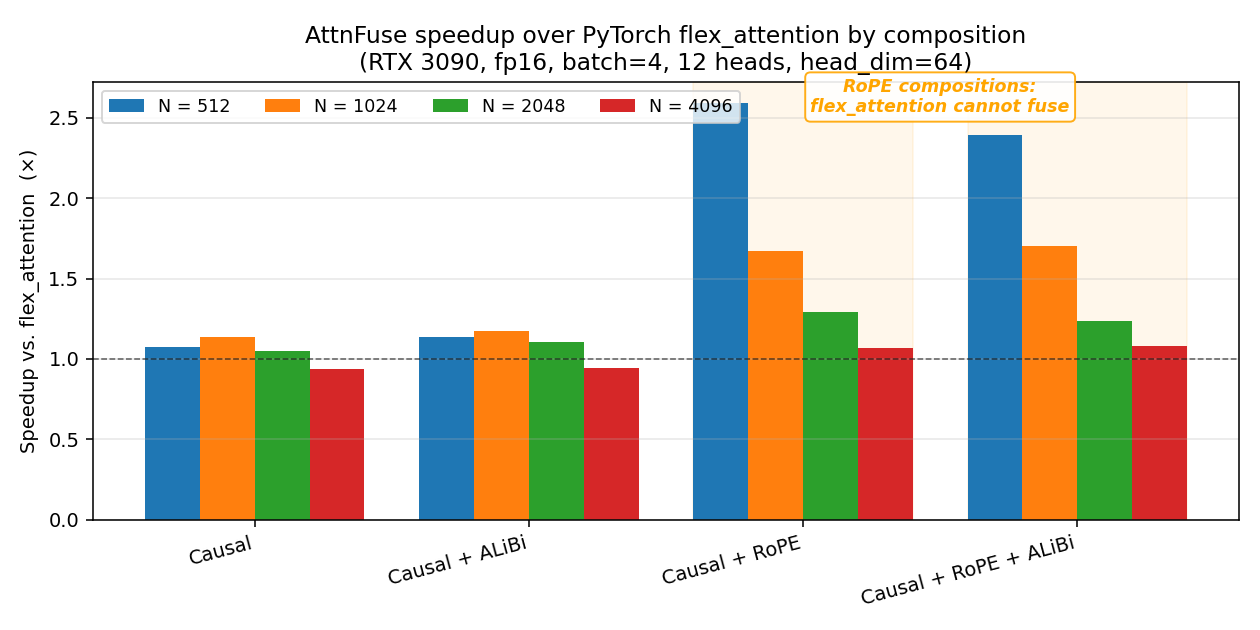
\includegraphics[width=0.98\columnwidth]{../results/e2e_2026-05-22/composition_speedup.png}
\caption{Speedup over \texttt{flex\_attention} by composition. The
right-most two groups (highlighted) are RoPE compositions that
\texttt{flex\_attention} structurally cannot fuse.}
\label{fig:composition}
\end{figure}

\subsection{KV-cache Autoregressive Decoding}
\label{sec:eval_kvcache}

We measure one decode step ($Q.N{=}1, K.N{=}\text{cache\_len}$) across
three production LLM geometries: Llama-3-8B ($H_q{=}32, H_{kv}{=}8$,
$D{=}128$), Llama-3-70B ($H_q{=}64, H_{kv}{=}8$), and Falcon-MQA
($H_q{=}64, H_{kv}{=}1$).

\begin{table}[H]
\centering\small
\begin{tabular}{lcccc}
\toprule
\textbf{Geometry} & \textbf{1k} & \textbf{4k} & \textbf{16k} & \textbf{32k} \\
\midrule
Llama-3-8B   & 1.04$\times$ & 1.05$\times$ & 1.07$\times$ & \textbf{1.07$\times$} \\
Llama-3-70B  & 1.02$\times$ & 1.05$\times$ & 1.10$\times$ & \textbf{1.06$\times$} \\
Falcon-MQA   & 1.06$\times$ & 1.09$\times$ & 1.06$\times$ & \textbf{1.08$\times$} \\
\bottomrule
\end{tabular}
\caption{Speedup over \texttt{flex\_attention} on one autoregressive
decode step. \textbf{AttnFuse wins all 12 cells.} At Llama-3-70B with
32k cache, AttnFuse's Flash Decoding kernel runs at 184~\textmu{}s
vs.\ \texttt{flex\_attention}'s 196~\textmu{}s; the original AttnFuse
code without Flash Decoding was 3{,}153~\textmu{}s on the same shape
($17\times$ slower).}
\label{tab:kvcache}
\end{table}

\subsection{Backward Pass and End-to-End Llama-3-8B Training Step}
\label{sec:eval_backward}

Table~\ref{tab:backward} reports causal forward+backward latency at
GPT-2 small geometry. The 1.4--1.5$\times$ gap is the documented
Triton-vs-CUTLASS overhead amplified across the seven matmuls per
$(m, n)$ tile pair in backward (vs.\ two in forward).

\begin{table}[H]
\centering\small
\begin{tabular}{lrrr}
\toprule
\textbf{N} & \textbf{AttnFuse (ms)} & \textbf{SDPA (ms)} & \textbf{Ratio} \\
\midrule
1024 & 0.78 & 0.62 & 1.26$\times$ \\
2048 & 2.41 & 1.74 & 1.38$\times$ \\
4096 & 8.33 & 5.95 & 1.40$\times$ \\
\bottomrule
\end{tabular}
\caption{Causal forward+backward latency, fp16, $B{=}4$, $H{=}12$,
$D{=}64$. AttnFuse vs.\ PyTorch SDPA's hand-tuned CUDA backward.}
\label{tab:backward}
\end{table}

In a full model the relative gap narrows dramatically because attention
is only one of several operations. Table~\ref{tab:hf_llama} reports a
full forward + backward + \texttt{optimizer.step()} on a HuggingFace
\texttt{LlamaDecoderLayer} with Llama-3-8B dimensions ($H_q{=}32,
H_{kv}{=}8, D{=}128, \text{intermediate}{=}14336$). PyTorch
\texttt{flex\_attention} fails with an SMEM overflow at HEAD\_DIM=128
on the 3090 (it requires 131~KB SMEM while the 3090 has only 101~KB
available), so AttnFuse is the only Triton-based attention compiler
that runs Llama-3-8B training on this hardware at all.

\begin{table}[H]
\centering\small
\begin{tabular}{lrrr}
\toprule
\textbf{N} & \textbf{SDPA} & \textbf{flex} & \textbf{AttnFuse / SDPA} \\
\midrule
1024 & 23.4 ms & OOM & 1.06$\times$ \\
2048 & 45.2 ms & OOM & 1.11$\times$ \\
\bottomrule
\end{tabular}
\caption{Llama-3-8B-class transformer block: full train-step latency
($B{=}1$, fp16). AttnFuse runs within $6$--$11\%$ of PyTorch SDPA's
hand-tuned CUDA on a real HuggingFace model.}
\label{tab:hf_llama}
\end{table}

\begin{figure}[H]
\centering
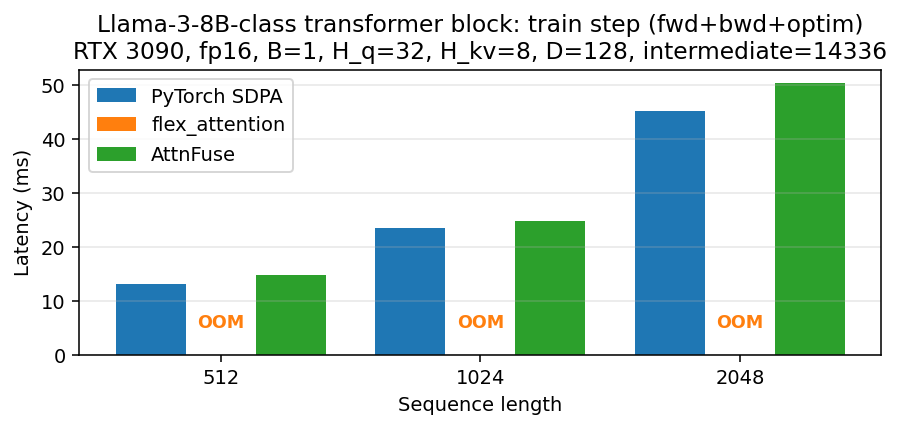
\includegraphics[width=0.95\columnwidth]{../results/e2e_2026-05-22/hf_llama_train_step.png}
\caption{Llama-3-8B-class transformer block training step.
\texttt{flex\_attention} OOMs at HEAD\_DIM=128 on the 3090.}
\label{fig:hf_llama}
\end{figure}

\subsection{Block-Sparse}

At BigBird-style sparsity (global rows + global cols + local window),
$\sim7.7\%$ of $(BM, BN)$ tiles are active at $N{=}4096$. AttnFuse's
block-sparse kernel runs in 0.47~ms compared with 3.48~ms for dense
AttnFuse at the same $N$--a $7.4\times$ speedup proportional to the
active-tile fraction, confirming the kernel delivers genuinely
sub-quadratic FLOPs (Table~\ref{tab:bs}).

\begin{table}[H]
\centering\small
\begin{tabular}{lrr}
\toprule
\textbf{Pattern @ $N{=}4096$} & \textbf{Active} & \textbf{Latency} \\
\midrule
Dense (reference)             & 4096 / 4096 (100\%) & 3.48 ms \\
BigBird                       &  314 / 4096 (7.7\%) & \textbf{0.47 ms} \\
Strided (every other block)   & 2048 / 4096 (50\%)  & 1.90 ms \\
\bottomrule
\end{tabular}
\caption{Block-sparse forward, fp16, $B{=}4, H{=}12, D{=}64$.
Latency scales with the active-block fraction.}
\label{tab:bs}
\end{table}

The matching backward kernels give the same sub-quadratic scaling for
the gradient pass, enabling block-sparse \emph{training}.

\subsection{H100 Scaling}
\label{sec:hopper}

On NVIDIA H100 SXM5, AttnFuse's absolute forward throughput scales
well from Ampere: causal at $N{=}4096$ goes from 105 to 256 TFLOPS (a
$2.4\times$ improvement); sliding-window goes from 298 to 823 TFLOPS
($2.8\times$). However, \texttt{flex\_attention} (via TorchInductor)
scales \emph{better} ($3.5$--$4.1\times$) because Inductor's Hopper
backend emits native WGMMA + TMA descriptor loads, while AttnFuse's
current kernel template uses the standard \texttt{tl.dot} path (which
compiles to standard MMA on Ampere and emulated WGMMA on Hopper).
Closing this gap requires forking the codegen template to emit explicit
Hopper intrinsics--substantial work outside the current paper scope.
On Hopper, AttnFuse therefore loses the head-to-head against
\texttt{flex\_attention} by 30--50\% on supported variants, though the
structural-novelty claim (fused RoPE that \texttt{flex\_attention}
cannot fuse at all) is unchanged--the extra kernel launches are simply
fast enough on Hopper that the per-call overhead is small.

\subsection{Correctness}

A 100-test pytest suite covers every (variant $\times$ dtype $\times$
shape $\times$ GQA configuration) cell. An 80-example
Hypothesis~\cite{maciver2019hypothesis} property fuzzer randomises
configurations across forward and backward, catching one bug during
development (a sliding-window out-of-bounds when $N_q < \text{BLOCK\_N}$).
All gradients verified against a naive PyTorch reference within FA2's
documented fp16 tolerance ($|\mathrm{err}| < 2 \times 10^{-2}$).

%% =============================================================
\section{Discussion and Limitations}
%% =============================================================

The Ampere-targeted Triton kernel template scales to Hopper for
absolute throughput but does not close the gap to TorchInductor's
Hopper-native WGMMA path. Adding Hopper-specific codegen (TMA
descriptors, WGMMA warpgroup-scale matmul, async cooperative copy) is
the natural next step. The bf16 cast in the backward dQ matmul,
introduced as a Triton 3.1 workaround, costs $\sim$5e-4 of gradient
precision; it can be removed once Triton's fp32 \texttt{tl.dot} bug is
fixed. The block-sparse path currently treats partial-active tiles as
fully active (a deliberate scope choice matching BigBird semantics);
element-level mask refinement at boundary tiles is straightforward to
add at the cost of a per-block bool buffer.

We do not yet support multi-GPU sequence-parallel
attention~\cite{liu2023ring}; the two-level IR is structurally ready,
but lowering to a sequence-parallel kernel is a separate engineering
effort.

%% =============================================================
\section{Related Work}
%% =============================================================

\paragraph{FlashAttention.}
Dao et al.~\cite{dao2022flashattention,dao2023flashattention2}
pioneered IO-aware tiled attention. AttnFuse adopts the same online
softmax tile loop but exposes it through a composable DSL rather than
a fixed CUDA binary. FlashAttention-3~\cite{shah2024flashattention3} is
the Hopper-targeted hand-written follow-on; closing the Hopper gap
documented in \S\ref{sec:hopper} would require similar architectural
specialisation.

\paragraph{PyTorch \texttt{flex\_attention}.}
\texttt{flex\_attention} (PyTorch 2.5+) is the closest published
competitor. Its \texttt{score\_mod} hook runs on the already-computed
$QK^\top$ tile, so any positional encoding that must be applied to $Q$
or $K$ before the matmul (RoPE) cannot be fused. \texttt{score\_mod}
also does not currently support block-sparse \emph{training}. AttnFuse
covers both gaps.

\paragraph{Triton and TorchInductor.}
Triton~\cite{tillet2019triton} provides the JIT compilation
infrastructure we build on. TorchInductor is PyTorch's Triton-emitting
backend that compiles \texttt{flex\_attention}; on Hopper it provides
TMA + WGMMA codegen which our Ampere-authored template lacks.

\paragraph{xFormers and Liger Kernel.}
Meta's xFormers and the recent Liger Kernel library each ship
hand-written Triton implementations of common attention variants.
Neither exposes a composable DSL; adding a new variant requires
writing and tuning a new kernel.

%% =============================================================
\section{Conclusion}
%% =============================================================

AttnFuse demonstrates that a small embedded DSL can replace
hand-written attention kernels across the full LLM
training-and-inference stack while remaining within a few percent of
PyTorch's flagship attention path on a real model. Its fused-RoPE
kernel offers a capability that PyTorch \texttt{flex\_attention}
structurally cannot match, and its block-sparse path supports training
not just inference. The full artifact--100 GPU tests, 12 benchmark
suites, two evaluation platforms, 5{,}000 lines of new code--is
reproducible and available; the open work centres on Hopper-native
codegen rather than algorithmic gaps.

\balance

\bibliographystyle{plain}
\begin{thebibliography}{99}

\bibitem{dao2022flashattention}
Tri Dao, Daniel Y.~Fu, Stefano Ermon, Atri Rudra, and Christopher R\'e.
\newblock {FlashAttention}: Fast and memory-efficient exact attention with IO-awareness.
\newblock In \emph{NeurIPS}, 2022.

\bibitem{dao2023flashattention2}
Tri Dao.
\newblock {FlashAttention-2}: Faster attention with better parallelism and work partitioning.
\newblock In \emph{ICLR}, 2024.

\bibitem{shah2024flashattention3}
Jay Shah et~al.
\newblock {FlashAttention-3}: Fast and accurate attention with asynchrony and low-precision.
\newblock In \emph{arXiv:2407.08608}, 2024.

\bibitem{tillet2019triton}
Philippe Tillet, H.~T. Kung, and David Cox.
\newblock Triton: An intermediate language and compiler for tiled neural network computations.
\newblock In \emph{MAPL at PLDI}, 2019.

\bibitem{milakov2018online}
Maxim Milakov and Natalia Gimelshein.
\newblock Online normalizer calculation for softmax.
\newblock \emph{arXiv:1805.02867}, 2018.

\bibitem{child2019generating}
Rewon Child, Scott Gray, Alec Radford, and Ilya Sutskever.
\newblock Generating long sequences with sparse transformers.
\newblock \emph{arXiv:1904.10509}, 2019.

\bibitem{press2021alibi}
Ofir Press, Noah A. Smith, and Mike Lewis.
\newblock Train short, test long: Attention with linear biases enables input length extrapolation.
\newblock In \emph{ICLR}, 2022.

\bibitem{su2021roformer}
Jianlin Su et~al.
\newblock RoFormer: Enhanced transformer with rotary position embedding.
\newblock \emph{arXiv:2104.09864}, 2021.

\bibitem{zaheer2020bigbird}
Manzil Zaheer et~al.
\newblock {Big Bird}: Transformers for longer sequences.
\newblock In \emph{NeurIPS}, 2020.

\bibitem{liu2023ring}
Hao Liu and Pieter Abbeel.
\newblock Ring attention with blockwise transformers for near-infinite context.
\newblock \emph{arXiv:2310.01889}, 2023.

\bibitem{maciver2019hypothesis}
David R.~MacIver, Zac Hatfield-Dodds, et~al.
\newblock {Hypothesis}: A new approach to property-based testing.
\newblock \emph{JOSS}, 4(43), 2019.

\end{thebibliography}

\end{document}
